\chapter{Lucht, een mengsel van gassen}\label{ch:g4:air-a-mixture-of-gases}

Op een winderige dag trekt een vlieger aan zijn touw, en op het meer
bolt een zeil op en duwt een boot vooruit. Iets duwt ertegen, en toch is
er niets te zien. Dat iets is \omterm{def:g4:air-a-mixture-of-gases:air}{lucht}. We kunnen het niet zien, maar het
is overal om ons heen, het vult elke lege fles en elke kamer, en we
ademen het in bij elke ademhaling. Waar bestaat \omterm{def:g4:air-a-mixture-of-gases:air}{lucht} uit?

\begin{recall}
\omterm{def:g2:mixing-and-dissolving:mix}{Mengen} is verschillende dingen bij elkaar doen; wat we krijgen, is een
mengsel van die dingen, en bij het \omterm{def:g2:mixing-and-dissolving:mix}{mengen} gaat er niets verloren
(\cref{ch:g2:mixing-and-dissolving}).
\end{recall}

\begin{omfigure}

\includegraphics[width=0.6\linewidth]{images/book1/ai/g4-kite-day.jpg}

{\small Een vlieger en een zeil: \omterm{def:g4:air-a-mixture-of-gases:air}{lucht} kun je niet zien, maar ze duwt
wel.}
\end{omfigure}

\section{Lucht is overal om ons heen}

\begin{example}[Een omgekeerd glas]\label{ex:g4:air-a-mixture-of-gases:glass}
Een droog papieren zakdoekje wordt onder in een leeg glas gedrukt. Het
glas wordt omgekeerd en recht naar beneden in een kom water geduwd. Als
je het er weer uit haalt, is het zakdoekje nog droog. Het glas was niet
leeg: het zat vol \omterm{def:g4:air-a-mixture-of-gases:air}{lucht}, en de \omterm{def:g4:air-a-mixture-of-gases:air}{lucht} hield het water tegen.
\end{example}

\begin{omfigure}
\begin{tikzpicture}[font=\small, scale=1.3]
  \pic[transform shape] at (0,0) {trough};
  % the upturned glass, rim at y = 0.35, base at y = 2.35
  \fill[white] (-0.8,0.5) rectangle (0.8,0.95);
  \pic[transform shape, rotate=180] at (0,2.35) {beaker={0}{white}};
  % the tissue at the top, inside
  \fill[white, draw=black!45, rounded corners=1.5pt] (-0.4,2.33) -- (-0.3,2.05)
    -- (-0.1,2.12) -- (0.05,1.98) -- (0.25,2.1) -- (0.42,2.02) -- (0.45,2.33) -- cycle;
  \draw[<-, omProp, thick] (0.45,2.12) -- (2.4,2.5) node[right, text=black]
    {een droog zakdoekje};
  \draw[<-, omProp, thick] (0.3,1.2) -- (2.4,1.4) node[right, text=black]
    {lucht: die houdt het water tegen};
  \draw[<-, omProp, thick] (1.4,0.7) -- (2.4,0.55) node[right, text=black]
    {water};
\end{tikzpicture}

{\small Het glas wordt ondersteboven in het water geduwd. De \omterm{def:g4:air-a-mixture-of-gases:air}{lucht} die
erin opgesloten zit, houdt het water tegen, en het zakdoekje blijft
droog.}
\end{omfigure}


\begin{remark}[Lucht is een gas]\label{rem:g4:air-a-mixture-of-gases:gas}
\omterm{def:g4:air-a-mixture-of-gases:air}{Lucht} is een gas: het heeft geen eigen vorm en verspreidt zich zo dat
het elke ruimte vult. Toch is het materie, en een ballon vol \omterm{def:g4:air-a-mixture-of-gases:air}{lucht} weegt
een beetje meer dan dezelfde ballon leeg. Wat gassen zijn, en waarom ze
zich zo gedragen, staat in het natuurkundeboek.
\end{remark}

\section{Lucht is een mengsel}

\begin{definition}[Lucht]\label{def:g4:air-a-mixture-of-gases:air}
\emph{Lucht}\index{lucht} is het mengsel van gassen dat de aarde
omringt. Het is niet één enkel gas: er zijn verschillende gassen in
gemengd, en die kun je van elkaar scheiden.
\end{definition}

\begin{proposition}[Waar lucht uit bestaat]\label{prop:g4:air-a-mixture-of-gases:composition}
% ledger: air:N2, air:O2, air:Ar, air:trace, air:CO2, air:H2O
Zonder de waterdamp bestaat \omterm{def:g4:air-a-mixture-of-gases:air}{lucht} uit:
\begin{itemize}
  \item \textbf{stikstof}, ongeveer vier vijfde van de \omterm{def:g4:air-a-mixture-of-gases:air}{lucht};
  \item \textbf{zuurstof}, ongeveer een vijfde van de \omterm{def:g4:air-a-mixture-of-gases:air}{lucht};
  \item een beetje \textbf{argon}, ongeveer 1 deel op 100;
  \item heel weinig \textbf{koolstofdioxide}, ongeveer 4 delen op
        10\,000, en piepkleine hoeveelheden andere gassen.
\end{itemize}
In \omterm{def:g4:air-a-mixture-of-gases:air}{lucht} zit ook \textbf{waterdamp}, onzichtbaar: heel weinig op een
droge, koude dag, tot ongeveer 4 delen op 100 op een warme, vochtige dag.
\end{proposition}

\begin{example}[Honderd flessen lucht]\label{ex:g4:air-a-mixture-of-gases:hundred}
% ledger: air:N2, air:O2, air:Ar
Stel je 100 flessen droge \omterm{def:g4:air-a-mixture-of-gases:air}{lucht} voor, en de gassen van de \omterm{def:g4:air-a-mixture-of-gases:air}{lucht}
gesorteerd over aparte flessen. Ongeveer 78 flessen zouden stikstof
bevatten, 21 flessen zuurstof, en de laatste fles argon, met een paar
druppeltjes koolstofdioxide en andere gassen.
\end{example}

\begin{omfigure}
\begin{tikzpicture}[font=\small, x=0.42cm, y=0.42cm]
  \foreach \k in {0,...,99} {
    \pgfmathtruncatemacro\col{mod(\k,10)}
    \pgfmathtruncatemacro\row{9-int(\k/10)}
    \ifnum\k<78 \def\c{omDef!45}\else\ifnum\k<99 \def\c{red!45}\else\def\c{cyan!60}\fi\fi
    \fill[\c, draw=white, line width=0.8pt] (\col,\row) rectangle ++(1,1);
  }
  \fill[omDef!45] (12,8) rectangle ++(1,1);
  \node[anchor=west] at (13.3,8.5) {stikstof: 78 vakjes};
  \fill[red!45] (12,6) rectangle ++(1,1);
  \node[anchor=west] at (13.3,6.5) {zuurstof: 21 vakjes};
  \fill[cyan!60] (12,4) rectangle ++(1,1);
  \node[anchor=west, align=left] at (13.3,4.5) {argon, koolstofdioxide\\ en de rest: 1 vakje};
\end{tikzpicture}

{\small Honderd vakjes droge \omterm{def:g4:air-a-mixture-of-gases:air}{lucht}. Het vakje rechtsonder bevat het
argon, en het koolstofdioxide, dat te weinig is om apart te tekenen.}
\end{omfigure}

\begin{remark}[Namen van gassen]\label{rem:g4:air-a-mixture-of-gases:names}
Stikstof, zuurstof, argon en koolstofdioxide zijn namen van gassen. Ze
zijn allemaal kleurloos en hebben geen geur. Een later hoofdstuk laat
zien waar elk van hen uit bestaat, tot op de piepkleine deeltjes waaruit
alle materie is opgebouwd.
\end{remark}

\section{Wat we in- en uitademen}

\begin{proposition}[Uitgeademde lucht]\label{prop:g4:air-a-mixture-of-gases:breath}
% ledger: breath:O2, breath:CO2, breath:N2, air:O2, air:CO2
De \omterm{def:g4:air-a-mixture-of-gases:air}{lucht} die we uitademen, is niet de \omterm{def:g4:air-a-mixture-of-gases:air}{lucht} die we hebben ingeademd. Ons
lichaam neemt een deel van de zuurstof op en geeft koolstofdioxide en
waterdamp af:
\begin{itemize}
  \item van de ingeademde \omterm{def:g4:air-a-mixture-of-gases:air}{lucht} is ongeveer 21 deel op 100 zuurstof, maar
        van de uitgeademde \omterm{def:g4:air-a-mixture-of-gases:air}{lucht} nog maar ongeveer 16 deel op 100;
  \item koolstofdioxide gaat van ongeveer 4 delen op 10\,000 naar ongeveer
        4 delen op 100: zo'n honderd keer meer;
  \item de stikstof ademen we net zo uit als we hem hebben ingeademd.
\end{itemize}
\end{proposition}

\begin{omfigure}
\begin{tikzpicture}
\begin{axis}[ybar, width=0.8\linewidth, height=5.2cm, bar width=12pt,
    ymin=0, ymax=90, ylabel={delen op 100},
    symbolic x coords={nitrogen, oxygen, carbon dioxide}, xtick=data,
    xticklabels={stikstof, zuurstof, koolstofdioxide},
    tick label style={font=\small}, label style={font=\small},
    xticklabel style={text height=1.6ex, text depth=0.4ex},
    legend style={font=\small, at={(0.98,0.95)}, anchor=north east},
    nodes near coords, nodes near coords style={font=\footnotesize},
    enlarge x limits=0.25, axis lines*=left, ymajorgrids,
    grid style={gray!20}]
% ledger: air:N2, air:O2, air:CO2, breath:N2, breath:O2, breath:CO2 (rounded)
\addplot[fill=omDef!45, draw=omDef] coordinates
  {(nitrogen,78) (oxygen,21) (carbon dioxide,0)};
\addplot[fill=omProp!55, draw=omProp] coordinates
  {(nitrogen,78) (oxygen,16) (carbon dioxide,4)};
\legend{ingeademd, uitgeademd}
\end{axis}
\end{tikzpicture}

{\small Ingeademd en uitgeademd, in delen op 100 (zonder de waterdamp,
afgeronde getallen). Het koolstofdioxide van de ingeademde \omterm{def:g4:air-a-mixture-of-gases:air}{lucht}, 4 delen
op 10\,000, is te weinig om als staaf te laten zien.}
\end{omfigure}

\begin{example}[Een volle klas]\label{ex:g4:air-a-mixture-of-gases:room}
In een klein lokaal met de ramen dicht ademen dertig mensen de hele
ochtend koolstofdioxide uit. Beetje bij beetje bevat de \omterm{def:g4:air-a-mixture-of-gases:air}{lucht} in het
lokaal minder zuurstof en meer koolstofdioxide, en de mensen worden moe.
Als je de ramen openzet, komt er weer frisse \omterm{def:g4:air-a-mixture-of-gases:air}{lucht} binnen.
\end{example}

\begin{omfigure}
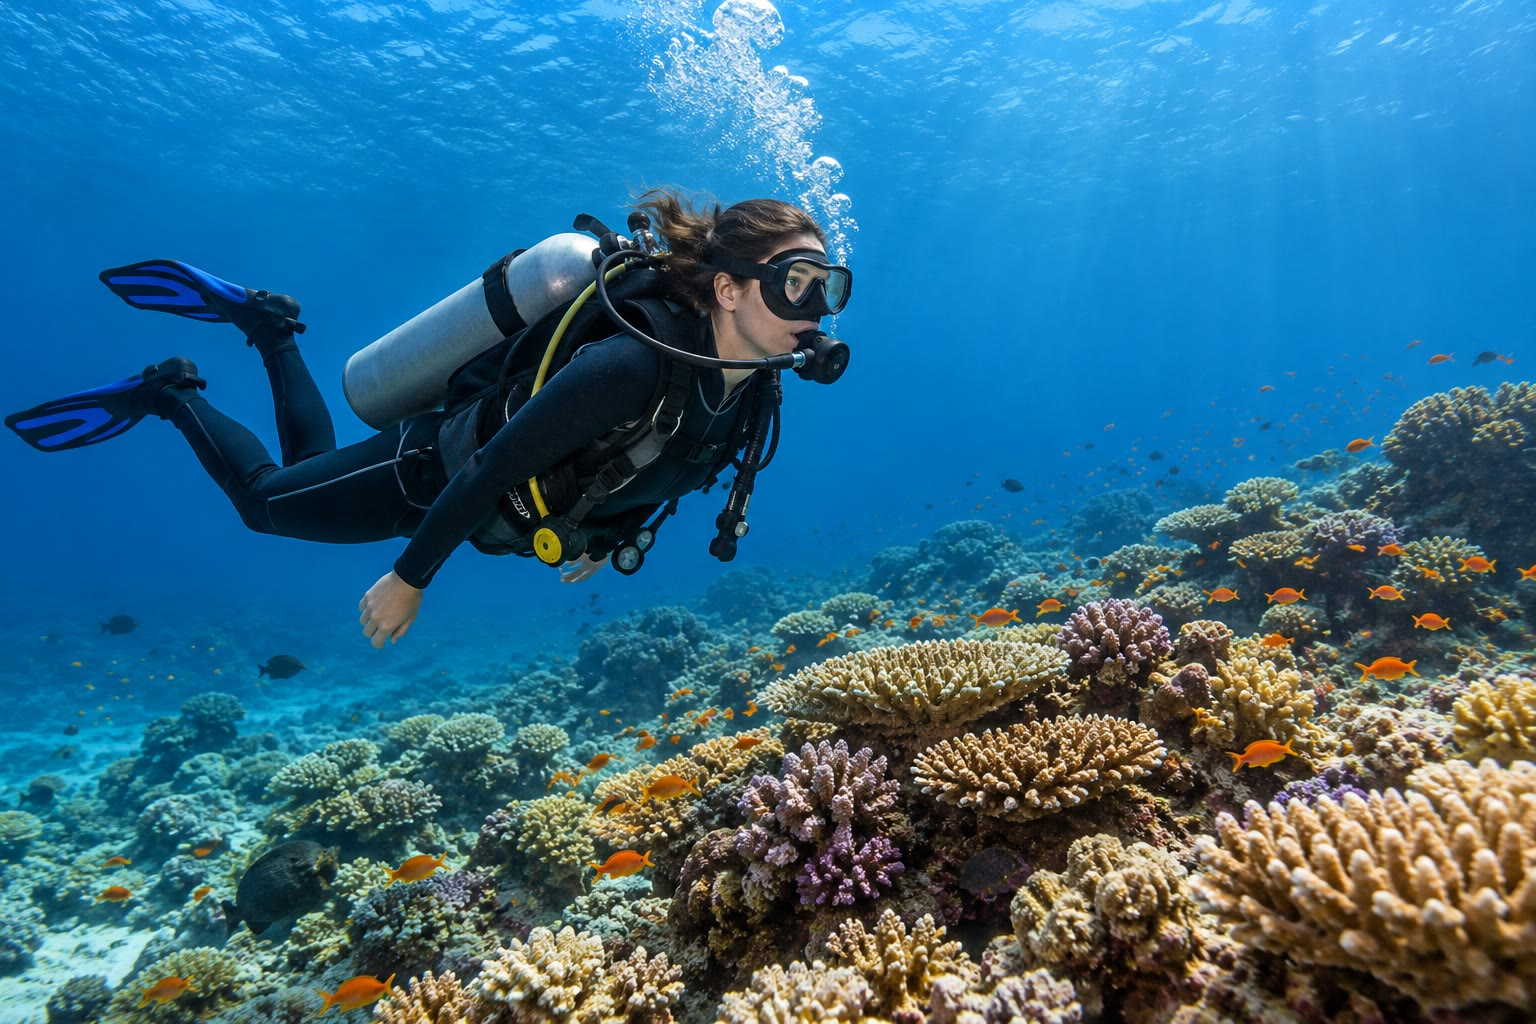
\includegraphics[width=0.55\linewidth]{images/book1/ai/g4-scuba-diver.jpg}

{\small Een duiker ademt \omterm{def:g4:air-a-mixture-of-gases:air}{lucht} uit de fles op zijn rug; de belletjes zijn
de uitgeademde \omterm{def:g4:air-a-mixture-of-gases:air}{lucht}.}
\end{omfigure}

\begin{remark}[Waarom duikers lucht ademen]\label{rem:g4:air-a-mixture-of-gases:diver}
De fles van een duiker is gevuld met \omterm{def:g4:air-a-mixture-of-gases:air}{lucht} die in een kleine ruimte is
samengeperst, niet met zuivere zuurstof: diep onder water zuivere
zuurstof ademen is gevaarlijk. De stikstof van de \omterm{def:g4:air-a-mixture-of-gases:air}{lucht} is er om de
zuurstof te verdunnen.
\end{remark}

\section{Zuurstof voor het leven en voor vuur}

\begin{proposition}[Levende wezens en vlammen verbruiken zuurstof]\label{prop:g4:air-a-mixture-of-gases:oxygen}
Van alle gassen van de \omterm{def:g4:air-a-mixture-of-gases:air}{lucht} is zuurstof het gas dat levende wezens en
vlammen nodig hebben. Dieren en mensen nemen het op als ze ademen; een
vlam haalt het uit de \omterm{def:g4:air-a-mixture-of-gases:air}{lucht} om zich heen. Groene planten geven bij
daglicht zuurstof terug aan de \omterm{def:g4:air-a-mixture-of-gases:air}{lucht}.
\end{proposition}

\begin{inthelab}[Een kaars onder een stolp]
De docent steekt een kaars aan op een tegel en laat er langzaam een
grote glazen stolp overheen zakken. De vlam wordt kleiner, flakkert en
gaat na een paar seconden uit: rond de vlam bevat de \omterm{def:g4:air-a-mixture-of-gases:air}{lucht} te weinig
zuurstof om hem te laten branden. Onder een stolp die twee keer zo groot
is, brandt de kaars ongeveer twee keer zo lang, omdat er ongeveer twee
keer zoveel \omterm{def:g4:air-a-mixture-of-gases:air}{lucht} is, en dus twee keer zoveel zuurstof om te verbruiken.
\end{inthelab}

\begin{omfigure}
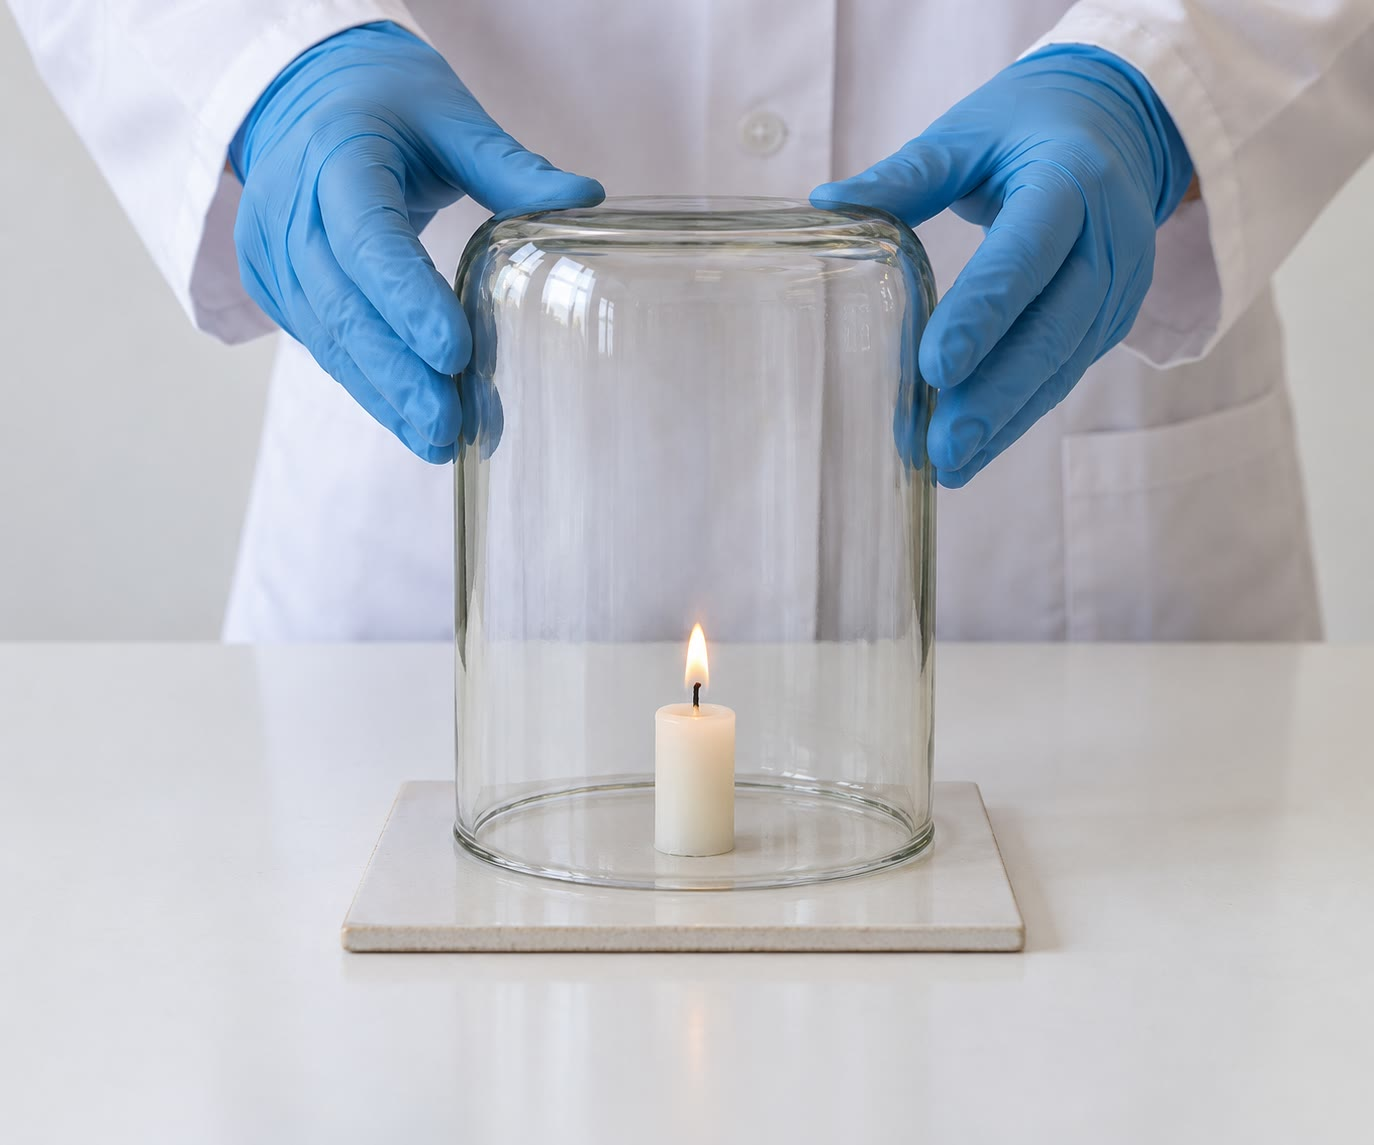
\includegraphics[width=0.5\linewidth]{images/book1/ai/g4-candle-jar-lab.jpg}

{\small Een kaars onder een glazen stolp gaat uit als er rond de vlam te
weinig zuurstof over is.}
\end{omfigure}

\begin{remark}[Stikstof brandt niet]\label{rem:g4:air-a-mixture-of-gases:nitrogen}
Stikstof is het grootste deel van de \omterm{def:g4:air-a-mixture-of-gases:air}{lucht}, en toch houdt het geen vlam
brandend en gebruikt ons lichaam het niet. Als \omterm{def:g4:air-a-mixture-of-gases:air}{lucht} helemaal uit
stikstof bestond, zouden we niet kunnen ademen en zou niets kunnen
branden.
\end{remark}

\section{Oefeningen}

\begin{exercise}[$\star$]\label{exo:g4:air-a-mixture-of-gases:1}
Is \omterm{def:g4:air-a-mixture-of-gases:air}{lucht} één enkel gas of een mengsel? Noem de twee belangrijkste gassen
van de \omterm{def:g4:air-a-mixture-of-gases:air}{lucht}.
\end{exercise}

\begin{exercise}[$\star$]\label{exo:g4:air-a-mixture-of-gases:2}
Welk deel van de \omterm{def:g4:air-a-mixture-of-gases:air}{lucht} is ongeveer stikstof? Welk deel is ongeveer
zuurstof?
\end{exercise}

\begin{exercise}[$\star$]\label{exo:g4:air-a-mixture-of-gases:3}
Hoeveel liter van 100 liter droge \omterm{def:g4:air-a-mixture-of-gases:air}{lucht} is ongeveer stikstof? Hoeveel
liter is ongeveer zuurstof?
\end{exercise}

\begin{exercise}[$\star$]\label{exo:g4:air-a-mixture-of-gases:4}
Een lege fles wordt ondersteboven in een bak water gezet. Waarom vult het
water de fles niet?
\end{exercise}

\begin{exercise}[$\star$]\label{exo:g4:air-a-mixture-of-gases:5}
Kijk naar het staafdiagram. Van welk gas zit er minder in de uitgeademde
\omterm{def:g4:air-a-mixture-of-gases:air}{lucht}? Van welk gas zit er meer in?
\end{exercise}

\begin{exercise}[$\star$]\label{exo:g4:air-a-mixture-of-gases:6}
Welk gas van de \omterm{def:g4:air-a-mixture-of-gases:air}{lucht} heeft een vlam nodig? Welk gas van de \omterm{def:g4:air-a-mixture-of-gases:air}{lucht} hebben
wij nodig als we ademen?
\end{exercise}

\begin{exercise}[$\star$]\label{exo:g4:air-a-mixture-of-gases:7}
Kijk naar de figuur met de 100 vakjes. Hoeveel vakjes zijn stikstof?
Hoeveel zijn geen stikstof?
\end{exercise}

\begin{exercise}[$\star$]\label{exo:g4:air-a-mixture-of-gases:8}
Waarom gaat een kaars onder een stolp na een tijdje uit?
\end{exercise}

\begin{exercise}[$\star$]\label{exo:g4:air-a-mixture-of-gases:9}
Hoeveel liter van 500 liter \omterm{def:g4:air-a-mixture-of-gases:air}{lucht} is ongeveer zuurstof? (Een vijfde van
de \omterm{def:g4:air-a-mixture-of-gases:air}{lucht} is zuurstof.)
\end{exercise}

\begin{exercise}[$\star\star$]\label{exo:g4:air-a-mixture-of-gases:10}
Waarom is het een goed idee om tussen de lessen door de ramen van een
lokaal open te zetten?
\end{exercise}

\begin{exercise}[$\star\star$]\label{exo:g4:air-a-mixture-of-gases:11}
Een kaars brandt 10 seconden onder een kleine stolp. Hoe lang zou hij
ongeveer branden onder een stolp met drie keer zoveel \omterm{def:g4:air-a-mixture-of-gases:air}{lucht}?
\end{exercise}
